% ---------------------------------------------------------------------------
%  Does Just-in-Time Defect Prediction Survive Realistic Evaluation?
%  Manuscript prepared for submission to IEEE Transactions on Software
%  Engineering. Compiles with pdflatex + bibtex (e.g. on Overleaf). To move it
%  into the official IEEEtran journal template, copy the body between
%  \begin{document} and \end{document} and switch natbib to IEEE numeric
%  citations (\bibliographystyle{IEEEtran}).
% ---------------------------------------------------------------------------
\documentclass[11pt,a4paper]{article}
\usepackage[utf8]{inputenc}
\usepackage[T1]{fontenc}
\usepackage{lmodern}
\usepackage[margin=2.5cm]{geometry}
\usepackage{amsmath,amssymb}
\usepackage{graphicx}
\usepackage{booktabs}
\usepackage{array}
\usepackage[round,authoryear]{natbib}
\usepackage{xcolor}
\usepackage[colorlinks=true,linkcolor=blue!50!black,citecolor=blue!50!black,urlcolor=blue!50!black]{hyperref}
\usepackage{caption}
\captionsetup{font=small,labelfont=bf}
\graphicspath{{figures/}}

\newcommand{\finding}[2]{\begin{quote}\noindent\textbf{Finding #1.} \emph{#2}\end{quote}}
\newcommand{\pthree}{P3\textsubscript{G90}}

\title{Does Just-in-Time Defect Prediction Survive Realistic Evaluation?\\[0.3em]
\large Time Order, Label Latency, and Review Effort on 321{,}288 Commits from Two Datasets}

\author{%
Farida Hisham Ghariani\textsuperscript{1}\\
{\small \href{mailto:fhmghariani@gmail.com}{fhmghariani@gmail.com}}\\
{\small ORCID: \href{https://orcid.org/0009-0003-8836-5118}{0009-0003-8836-5118}}
\and
Alla Khaled Almuqadimi\textsuperscript{2,*}\\
{\small \href{mailto:al3muqadimi@gmail.com}{al3muqadimi@gmail.com}}\\
{\small ORCID: \href{https://orcid.org/0009-0001-4590-4236}{0009-0001-4590-4236}}}
% NOTE: add the supervisor as a co-author here if he contributed to the
% design, analysis or writing (see the CRediT statement at the end).

\date{\small\textsuperscript{1,2}College of Computer Technology (CCTT), Postgraduate Program, MSc Computer Science, Tripoli, Libya\\[0.3em]
\textsuperscript{*}Corresponding author: \href{mailto:al3muqadimi@gmail.com}{al3muqadimi@gmail.com}}

\begin{document}
\maketitle

% ===========================================================================
\begin{abstract}
\noindent\textbf{Context.} Just-in-time software defect prediction (JIT-SDP) flags risky commits when they are submitted. Many reported results come from shuffled train/test splits and from labels that a team could not have known at training time, so they may not transfer to practice.

\noindent\textbf{Objective.} We quantify how chronological splitting, label-latency handling, class-imbalance treatment, and effort-aware evaluation change the measured performance and the ranking of standard classifiers.

\noindent\textbf{Method.} We run a controlled, leakage-checked experiment on two independent datasets. ApacheJIT contributes 13 Apache projects (93{,}871 commits). The dataset of Kamei et~al.\ contributes six projects written in C, C++, Perl, and Java (227{,}417 commits). Logistic regression, random forest, and XGBoost are compared with a prevalence baseline and an unsupervised inverse-churn baseline under three protocols: a random split (P1), a chronological split (P2), and a chronological split that withholds the last $G\in\{30,90,180\}$ days of unlabelled commits (P3). We add 495 rolling windows, each paired with a shuffled split of the \emph{same} commits, and use SHAP to study how stable feature importance is over time. In total we evaluate 4{,}801 model and baseline runs.

\noindent\textbf{Results.} Over the 19 projects, replacing P1 with \pthree{} lowers the median PR-AUC by 0.067 and F1 by 0.071 ($p<0.001$; Holm-adjusted $p\le0.003$ for every model), with a medium effect on MCC. The effect replicates in both datasets. Almost all of it comes from time ordering; the latency gap adds little. The size of the drop follows the lower observed defect prevalence of recent commits (Spearman $\rho\approx-0.75$), and prevalence-normalised PR-AUC does not drop. When the same commits are compared, a smaller genuine time-order penalty remains (0.024 PR-AUC overall; 0.037 in the Kamei data). Once decision thresholds are tuned on validation data, class weighting and under-sampling do not improve recall, and they give at most negligible F1 gains. XGBoost has the best average rank on PR-AUC. However, every classifier that ranks commits by raw risk loses to the inverse-churn baseline on Recall@20\% effort. Ranking by risk per changed line reverses this result in every model and in both datasets ($p<0.001$; large effect on the Kamei data). Change size is the dominant predictor in both datasets. Top-five feature rankings are stable in the Kamei data (median $\rho=0.71$) but not in ApacheJIT ($\rho=0.60$).

\noindent\textbf{Conclusions.} Random splits overstate JIT-SDP performance on two independent datasets. A large part of the measured gap reflects immature labels rather than weaker models, but a smaller genuine penalty for time ordering remains. We recommend time-ordered evaluation, reporting prevalence-normalised metrics, density-based ranking for review prioritisation, and monitoring of feature drift.

\medskip\noindent\textbf{Keywords:} Just-in-time defect prediction $\cdot$ Model validation $\cdot$ Verification latency $\cdot$ Class imbalance $\cdot$ Effort-aware evaluation $\cdot$ SHAP $\cdot$ Replication
\end{abstract}

% ===========================================================================
\section{Introduction}\label{sec:intro}

Most commits are harmless, but a minority introduce defects that are found only after integration, testing, or release. Just-in-time software defect prediction (JIT-SDP) estimates, at the moment a change is submitted, the probability that it will later be found to be defect-inducing \citep{mockus2000,kamei2013}. Reliable estimates would let teams concentrate review and testing effort where it matters most. Since \citet{kamei2013}, JIT-SDP has grown to include deep models \citep{hoang2019,hoang2020}, simpler but strong line-level approaches \citep{pornprasit2021}, online and cross-project learning \citep{tabassum2022,cabral2022}, and uncertainty estimation \citep{shahini2024}.

Much of this progress is measured under conditions that a development team cannot reproduce. First, commits are often shuffled before splitting, so information from the future leaks into training and performance is overestimated \citep{tantithamthavorn2017,falessi2020,song2023a}. Second, a commit is labelled defect-inducing only after a later fix is traced back to it, typically with an SZZ-style algorithm \citep{sliwerski2005}. At training time, recent commits that are in fact defective still look clean. This \emph{verification latency} makes training labels systematically incomplete \citep{cabral2019}. Third, defect-inducing commits are a minority. Accuracy and, to a lesser extent, ROC-AUC can therefore look good while a model misses most risky commits or saves little review effort \citep{yang2016,saito2015}.

These factors have mostly been studied in isolation, on one dataset, or with one protocol. There is little controlled evidence, obtained with one pipeline, one set of models, and more than one dataset, on how much each factor changes the conclusions drawn about standard, easily reproduced classifiers. This paper provides such evidence. We use two independent datasets: ApacheJIT \citep{keshavarz2022}, a recent large dataset of Apache projects, and the dataset of \citet{kamei2013}, which covers C, C++, Perl, and Java systems and was labelled with a different pipeline. We do not propose a new model. We measure how evaluation choices change what we conclude about existing ones, in line with the observation that simple models can match complex ones when evaluation is careful \citep{zeng2021}.

We address three research questions:
\begin{description}
\item[RQ1] How much does performance fall when a random split is replaced by a chronological split with label-latency handling?
\item[RQ2] Under realistic evaluation, which imbalance strategy and which model give the most useful results, and do they outperform simple baselines?
\item[RQ3] Which features contribute most to predictions, and are they stable across time windows?
\end{description}

For each question we stated a testable hypothesis before running the experiments (Section~\ref{sec:design}); rejecting a hypothesis is a reportable outcome.

\paragraph{Contributions.}
\begin{enumerate}
\item A reproducible, leakage-checked evaluation protocol. It combines chronological splitting with explicit label-latency handling and applies them identically to three classifiers, two baselines, and two datasets. Each leakage rule has an automated test.
\item Replicated evidence on 19 projects from two datasets that random splitting overstates PR-AUC, F1, and MCC. A decomposition shows that time ordering, not the latency gap, causes almost all of the difference.
\item A new analysis that separates the realism penalty into two parts. The first comes from label immaturity: the per-project drop tracks the lower observed defect prevalence of recent commits, and prevalence-normalised PR-AUC does not drop. The second is a genuine time-order penalty, measured with a paired design on identical commits. That penalty is small, and it is larger in the older, multi-language dataset.
\item Evidence that, with validation-tuned thresholds, rebalancing does not improve recall. Supervised models beat the strong unsupervised baseline on effort-aware recall only when they rank commits by risk per changed line, and they do so in both datasets.
\item A SHAP analysis over 495 rolling windows. It shows that change size dominates in both datasets, while the stability of the remaining top features depends on the dataset.
\end{enumerate}

Section~\ref{sec:related} reviews related work, Section~\ref{sec:design} describes the study design, Section~\ref{sec:results} answers the research questions, Section~\ref{sec:discussion} discusses implications, Section~\ref{sec:threats} discusses threats to validity, and Section~\ref{sec:conclusion} concludes.

% ===========================================================================
\section{Background and Related Work}\label{sec:related}

\paragraph{Foundations of JIT-SDP.}
\citet{mockus2000} introduced change-level risk prediction. \citet{kamei2013} defined the widely used change metrics (size, diffusion, history, and developer experience), released six projects as a benchmark, showed that logistic regression is a competitive baseline, and introduced effort-aware evaluation in which effort is approximated by lines changed. Labels are usually produced with SZZ \citep{sliwerski2005}, which traces a fix back to the change that last touched the faulty lines. SZZ labels are useful but noisy, and data-collection choices change results \citep{herbold2022}. ApacheJIT \citep{keshavarz2022} provides about 106 thousand recent commits from Apache projects with commit-level metrics and SZZ-based labels.

\paragraph{Validation and time.}
\citet{tantithamthavorn2017} showed that the choice of model validation technique changes performance estimates for defect prediction. \citet{falessi2020} showed that order-preserving techniques such as walk-forward validation give more accurate estimates than cross-validation or bootstrap, and that defect rates change over time in most projects. \citet{bangash2020} found that conclusions about cross-project defect prediction models are not stable over time. For JIT-SDP, \citet{song2023a} analysed when retrospective evaluation procedures are valid, and \citet{mcintosh2018} showed that the properties of fix-inducing changes drift as systems evolve.

\paragraph{Verification latency.}
\citet{cabral2019} studied class-imbalance evolution together with verification latency in online JIT-SDP. \citet{cabral2022} showed that concept drift and latency together harm the stability of predictive performance, and \citet{song2023b} proposed practical human labelling to reduce the cost of waiting for labels. Outside JIT-SDP, \citet{jimenez2019} showed that ignoring real-world labelling time inflates vulnerability-prediction results. Our P3 protocol follows this line: commits whose label is not yet observable at the training cut-off are treated as unlabelled and withheld, not relabelled as clean.

\paragraph{Imbalance and effort-aware evaluation.}
\citet{tantithamthavorn2020} showed that class rebalancing can improve recall but shifts probability estimates and model interpretation. \citet{yang2016} found that simple unsupervised models that rank changes by a single metric can beat supervised models on effort-aware measures. \citet{fu2017} and \citet{huang2019} revisited this claim and showed that supervised models remain competitive under some settings. We use an inverse-churn ranker in this spirit as our unsupervised baseline, and we report both raw and density-based rankings of supervised models.

\paragraph{Explainability and drift.}
SHAP values \citep{lundberg2017} attribute a prediction to input features and are widely used to explain tree ensembles. Together with the drift results of \citet{mcintosh2018}, they allow the temporal stability of feature importance to be measured directly.

\paragraph{Positioning.}
Recent work mainly proposes new models \citep{hoang2019,hoang2020,pornprasit2021,sahar2024,vandinter2023}. Our study is complementary. It is a controlled, two-dataset measurement of how realistic evaluation conditions alter the conclusions drawn about standard classifiers, using one pipeline and paired tests.

% ===========================================================================
\section{Study Design}\label{sec:design}

All models share the same features, preprocessing, and test sets within a dataset; only the factor under study (protocol, imbalance strategy, or model) changes between runs. Random seeds are fixed. Every table and figure in this paper is regenerated by two commands (Section~\ref{sec:repro}).

\subsection{Datasets and readiness gate}\label{sec:data}

Before modelling, each dataset had to pass a pre-registered \emph{readiness gate}: (1) usable commit timestamps, (2) the required change metrics, (3) binary labels, (4) enough positive and negative examples, and (5) enough information to implement at least one label-latency protocol. Both datasets pass. Neither provides fix-commit timestamps, so label latency is approximated with a gap (Section~\ref{sec:protocols}). Table~\ref{tab:datasets} summarises the datasets.

\begin{table}[t]
\centering
\caption{Datasets. Commits and prevalence refer to the retained projects.}
\label{tab:datasets}
\small
\begin{tabular}{lll}
\toprule
 & ApacheJIT \citep{keshavarz2022} & Kamei et al.\ \citep{kamei2013} \\
\midrule
Projects (retained / total) & 13 / 15 & 6 / 6 \\
Retained commits & 93{,}871 & 227{,}417 \\
Period & 2003--2019 & 1996--2010 \\
Languages & Java (Apache ecosystem) & C, C++, Perl, Java \\
Defect prevalence & 26.5\% (all 15 projects) & 12.3\% \\
Labelling & SZZ (2022 pipeline) & SZZ variant (2013 pipeline) \\
Churn metrics & absolute lines & normalised by lines in touched files \\
Rolling windows & 344 & 151 \\
\bottomrule
\end{tabular}
\end{table}

\paragraph{ApacheJIT.} We use \texttt{apachejit\_total.csv} (SHA-256 \texttt{5097cbbb\ldots ddbed4e0}). It contains 106{,}674 commits from 15 projects; 26.5\% are defect-inducing. There are no missing values and no duplicated commit identifiers.

\paragraph{Kamei et al.} We use the six projects released by \citet{kamei2013} (Bugzilla, Columba, Eclipse JDT, Eclipse Platform, Mozilla, PostgreSQL), as distributed in the replication package of \citet{yang2016} and \citet{fu2017} (combined SHA-256 \texttt{db1ccef8\ldots 7c5caa09}). The 227{,}417 commits have no missing values and no duplicated identifiers. In this dataset lines added and deleted are normalised by the lines in the touched files before the change (LT). We therefore use the normalised values as model features and reconstruct absolute churn, $(\texttt{la}+\texttt{ld})\cdot\texttt{lt}$, as the effort proxy, following \citet{yang2016}.

\paragraph{Exclusion rule.} The rule was fixed before modelling: a project is retained only if its chronological 70/30 split contains at least 50 commits of each class in both the training and the test part. All six Kamei projects pass. Two ApacheJIT projects are excluded. \texttt{apache/zookeeper} has only 35 defect-inducing commits in its test part. \texttt{apache/hadoop} has \emph{no} defect-inducing commit among 11{,}964 commits, whereas its sub-projects \texttt{hadoop-hdfs} and \texttt{hadoop-mapreduce} have 76\% and 63\%; we treat this as a labelling artefact of the repository split. The 19 retained projects contain 321{,}288 commits.

\paragraph{Label maturity.} Figure~\ref{fig:prevyear} shows that the share of defect-inducing commits falls towards the end of both datasets. Recent commits have had less time for their defects to be discovered, so their observed labels are incomplete. In 15 of the 19 projects the test part of the chronological split has a lower observed prevalence than the training part. This affects any evaluation in which the test set is newer than the training set, and it is central to RQ1.

\begin{figure}[t]
\centering
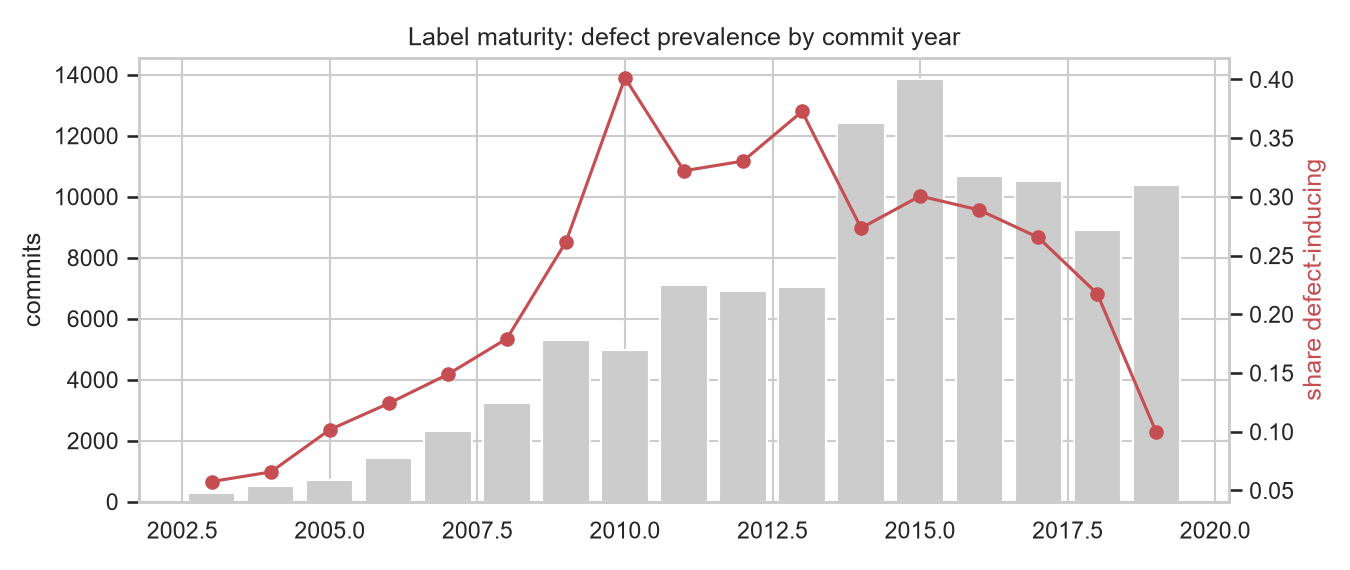
\includegraphics[width=0.49\linewidth]{data_prevalence_by_year.png}\hfill
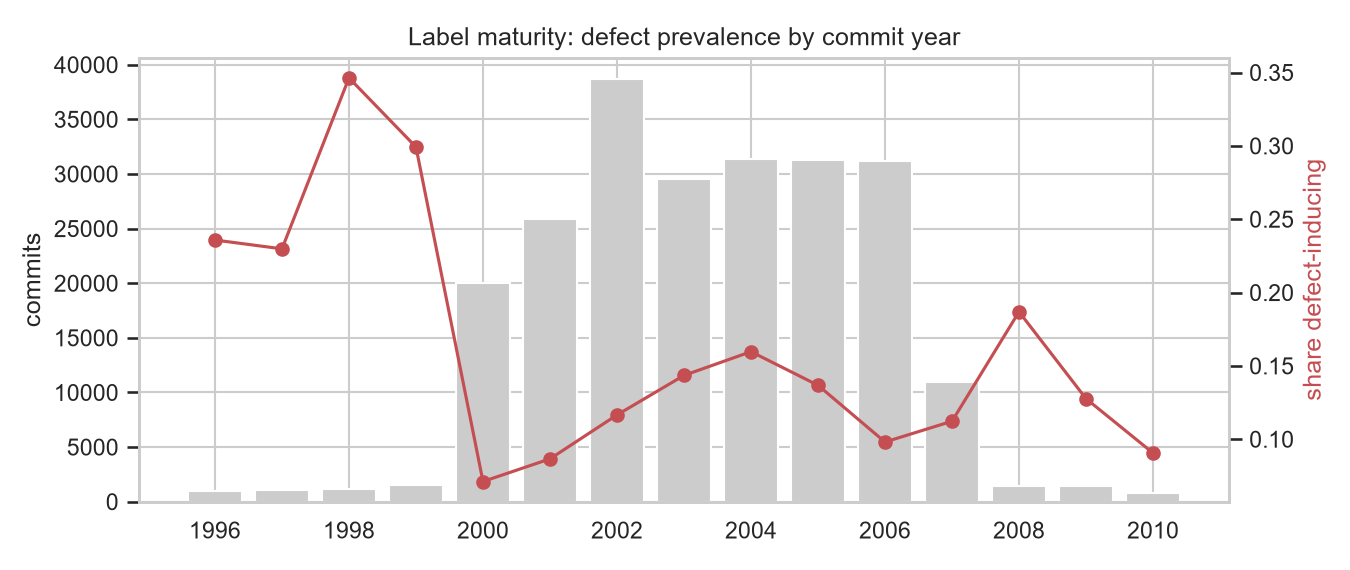
\includegraphics[width=0.49\linewidth]{k_data_prevalence_by_year.png}
\caption{Commits per year (bars) and share labelled defect-inducing (line). Left: ApacheJIT; right: Kamei et al. The falling share near the end of each dataset is consistent with labels that have not yet matured.}
\label{fig:prevyear}
\end{figure}

\subsection{Features and leakage rules}\label{sec:features}

We use the 13 change-level metrics that are common to both datasets and available at commit time. They are lines added (\texttt{la}) and deleted (\texttt{ld}); the numbers of files (\texttt{nf}), directories (\texttt{nd}), and subsystems (\texttt{ns}); the entropy of the change (\texttt{ent}); the number of previous developers (\texttt{ndev}); the average age of the modified files (\texttt{age}); the number of unique changes (\texttt{nuc}); developer experience (\texttt{aexp}), recent experience (\texttt{arexp}), and subsystem experience (\texttt{asexp}); and the \texttt{fix} indicator. The \texttt{fix} indicator states whether the commit is itself a bug fix. It is derived from the commit's own message and is therefore known at commit time. Identifiers, project names, timestamps, and the \texttt{year} field are forbidden as features.

Preprocessing is wrapped in a single transformer that is fitted on training data only and applied unchanged to validation and test data. It applies $\log(1+x)$ to skewed count metrics. For logistic regression only, it also removes one feature of each pair with Spearman $|\rho|>0.8$ and standardises the remaining features. Tree models receive all 13 transformed features, so that SHAP rankings are comparable across windows.

Every split passes an automated check before training. The check confirms that no forbidden feature is used, that no commit appears in both training and test data, that training timestamps do not exceed test timestamps in time-ordered protocols, and that the latency gap is respected. Twelve unit tests exercise these rules, the protocols, and the metrics.

\subsection{Evaluation protocols}\label{sec:protocols}

Each project is ordered by author date. We follow a \emph{label-availability rule}: a commit whose defect status is not yet observable at the training cut-off is treated as unlabelled and removed from the supervised training set. It is never relabelled as clean.

\begin{description}
\item[P1 -- Random.] Stratified random 70/30 split, repeated with three seeds and averaged. It is the retrospective reference for RQ1.
\item[P2 -- Chronological.] The earliest 70\% of commits are used for training and the latest 30\% for testing.
\item[P3 -- Chronological with latency gap.] The same test commits as P2, but commits authored in the $G$ days before the first test commit are withheld from training. $G=90$ is the default (\pthree); $G=30$ and $G=180$ are sensitivity settings. The median number of withheld commits per project is 67, 165, and 355 in ApacheJIT, and 339, 981, and 2{,}038 in the Kamei data.
\item[Rolling windows.] Train on 12 months, skip a 90-day gap, test on the next 3 months, and move forward by 3 months. A window is kept if its training part has at least 30 commits of each class and its test part at least 10. This yields 495 windows (344 in ApacheJIT, 151 in the Kamei data). Each window is paired with a \emph{shuffled counterpart}: the same training and test commits are pooled and re-split at random with the same test size. Because both members of a pair contain exactly the same commits, the comparison isolates the effect of time order from differences in test-set composition.
\end{description}

We also repeat P1--P3 on the pooled data of each dataset, ordered by global time.

\subsection{Models and baselines}\label{sec:models}

We compare logistic regression (LR), the classical JIT baseline \citep{kamei2013}; random forest (RF, 200 trees) \citep{breiman2001}; and XGBoost (XGB, 300 rounds, subsample and column sample 0.8) \citep{chen2016}. Two baselines are reported next to every result. The \emph{prevalence} baseline outputs the training base rate for every commit; its PR-AUC equals the chance level, and it predicts the majority class. The unsupervised \emph{inverse-churn} baseline, which we label LT for ``lines touched'' (not to be confused with Kamei's LT metric), ranks commits by $1/\text{churn}$ in the spirit of \citet{yang2016}. It flags the same share of commits as the training prevalence, using a threshold taken from training scores.

Hyper-parameters are tuned on training data only, by mean PR-AUC over three folds. The grids are: LR $C\in\{0.01,0.1,1,10\}$; RF maximum depth $\in\{\text{none},12\}\times$ minimum leaf size $\in\{1,5\}$; and XGB maximum depth $\in\{3,6\}\times$ learning rate $\in\{0.03,0.1\}$. For P2 and P3 the folds are time-ordered, so each fold validates on data later than its training data; for P1 they are stratified random folds. Rolling windows use fixed mid-grid settings to keep the 2{,}970 window fits tractable.

\subsection{Imbalance strategies and decision thresholds}\label{sec:imbalance}

Under \pthree{} we compare three strategies: (i) no treatment; (ii) class weighting, with balanced weights for LR and RF and $\texttt{scale\_pos\_weight}=n_{\text{clean}}/n_{\text{buggy}}$ for XGB; and (iii) random under-sampling applied inside the training pipeline only \citep{lemaitre2017}. Class weighting is the default strategy elsewhere, and test data are never resampled. In every run the model is first fitted on the first 80\% of the training data. The F1-optimal threshold is then selected on the remaining 20\%, which is the most recent 20\% for P2 and P3. Finally the model is refitted on all training data and that threshold is kept.

\subsection{Metrics}\label{sec:metrics}

At the validation threshold we report precision, recall, F1, MCC, and the confusion matrix. We also report PR-AUC (average precision), which is the primary metric \citep{saito2015}, ROC-AUC, and the Brier score. \emph{Recall@20\% effort} is the share of defect-inducing commits found when commits are inspected in ranked order until 20\% of the total churn has been reviewed. $P_{\text{opt}}$ \citep{kamei2013} compares the area under the cumulative effort--recall curve of a ranking with those of the optimal and the worst rankings. Supervised models are ranked in two ways: by predicted risk, and by risk density (risk divided by churn). Ties are broken at random, because breaking ties by effort would silently turn a constant-score model into the inverse-churn baseline; a unit test guards against this. Test-set prevalence differs between protocols (Figure~\ref{fig:prevyear}), so we also report \emph{PR-AUC lift}, which is PR-AUC divided by test prevalence, i.e.\ the ratio to the chance level.

\subsection{Statistical analysis}\label{sec:stats}

Paired comparisons use the Wilcoxon signed-rank test, one-sided for directional hypotheses and two-sided otherwise, with $\alpha=0.05$. Holm correction \citep{holm1979} is applied within families of per-model tests. Effect sizes use Cliff's $\delta$ with the thresholds of \citet{romano2006}: negligible $<0.147$, small $<0.33$, medium $<0.474$, and large otherwise. To compare several rankers over several projects we use the Friedman test followed by the Nemenyi post-hoc test and its critical difference (CD) \citep{demsar2006}. Every test is reported over all 19 projects and per dataset. For pooled results we report 95\% bootstrap confidence intervals of PR-AUC from 1{,}000 resamples.

\paragraph{Hypotheses.}
\textbf{H1}: PR-AUC and F1 under \pthree{} are significantly lower than under P1.
\textbf{H2}: (a) class weighting improves recall and F1 relative to no treatment without lowering PR-AUC, and (b) at least one ML model outperforms the inverse-churn baseline on Recall@20\% effort.
\textbf{H3}: the ranking of the top five features by mean $|\text{SHAP}|$ is stable across windows, defined as a median Spearman $\rho\ge0.7$ between consecutive windows.

\subsection{Explainability}\label{sec:shap}

For every realistic rolling window we compute TreeSHAP values \citep{lundberg2017} of the XGB model on up to 400 test commits and rank the 13 features by mean $|\text{SHAP}|$. For consecutive windows of the same project we compute three quantities: Spearman's $\rho$ over the union of the two top-five sets, Spearman's $\rho$ over all 13 features, and the Jaccard overlap of the two top-five sets. Global importance is computed for the pooled \pthree{} XGB model of each dataset on 2{,}000 test commits. Explanations describe model behaviour and are not causal claims.

\subsection{Implementation and reproducibility}\label{sec:repro}

The pipeline is written in Python 3.12 with scikit-learn 1.9 \citep{pedregosa2011}, XGBoost 3.4, imbalanced-learn 0.14, SHAP 0.54, and SciPy 1.18. The command \texttt{python run\_all.py --dataset \{apachejit|kamei\}} validates a dataset, runs all its evaluations, and writes its tables and figures. On a 12-core workstation this takes 19 minutes for ApacheJIT and 36 minutes for the Kamei data. The command \texttt{python cross\_dataset.py} then re-tests all hypotheses over the 19 projects. A command-line prototype (\texttt{predict.py}) applies a persisted model to a feature record and returns a risk score and a Low/Medium/High level, using thresholds derived from validation data.

% ===========================================================================
\section{Results}\label{sec:results}

\subsection{RQ1: How much does performance fall under realistic evaluation?}\label{sec:rq1}

Table~\ref{tab:rq1} and Figure~\ref{fig:rq1} report median performance per dataset. In both datasets, moving from P1 to \pthree{} lowers the median PR-AUC of every model. For example, XGB falls from 0.834 to 0.715 in ApacheJIT and from 0.552 to 0.453 in the Kamei data. F1 and MCC follow the same pattern. Absolute values are lower in the Kamei data, whose prevalence is lower (12.3\%), but PR-AUC lift is similar (2.1--2.9).

\begin{table}[t]
\centering
\caption{Median performance per dataset (class weighting). Lift = PR-AUC / test prevalence.}
\label{tab:rq1}
\small
\begin{tabular}{llrrrrrrrr}
\toprule
 & & \multicolumn{4}{c}{ApacheJIT (13 projects)} & \multicolumn{4}{c}{Kamei et al.\ (6 projects)} \\
\cmidrule(lr){3-6}\cmidrule(lr){7-10}
Protocol & Model & PR-AUC & Lift & F1 & MCC & PR-AUC & Lift & F1 & MCC \\
\midrule
P1 & LR  & 0.790 & 1.87 & 0.724 & 0.516 & 0.454 & 2.17 & 0.470 & 0.285 \\
   & RF  & 0.809 & 2.00 & 0.732 & 0.561 & 0.541 & 2.67 & 0.515 & 0.363 \\
   & XGB & 0.834 & 2.00 & 0.740 & 0.578 & 0.552 & 2.76 & 0.527 & 0.370 \\
\midrule
P2 & LR  & 0.700 & 2.53 & 0.627 & 0.393 & 0.369 & 2.15 & 0.418 & 0.251 \\
   & RF  & 0.657 & 2.45 & 0.626 & 0.399 & 0.451 & 2.75 & 0.429 & 0.295 \\
   & XGB & 0.715 & 2.52 & 0.642 & 0.454 & 0.469 & 2.93 & 0.438 & 0.312 \\
\midrule
\pthree & LR  & 0.689 & 2.53 & 0.603 & 0.396 & 0.363 & 2.15 & 0.412 & 0.240 \\
   & RF  & 0.650 & 2.38 & 0.613 & 0.410 & 0.432 & 2.69 & 0.447 & 0.292 \\
   & XGB & 0.715 & 2.51 & 0.626 & 0.443 & 0.453 & 2.86 & 0.428 & 0.311 \\
\bottomrule
\end{tabular}
\end{table}

\begin{figure}[t]
\centering
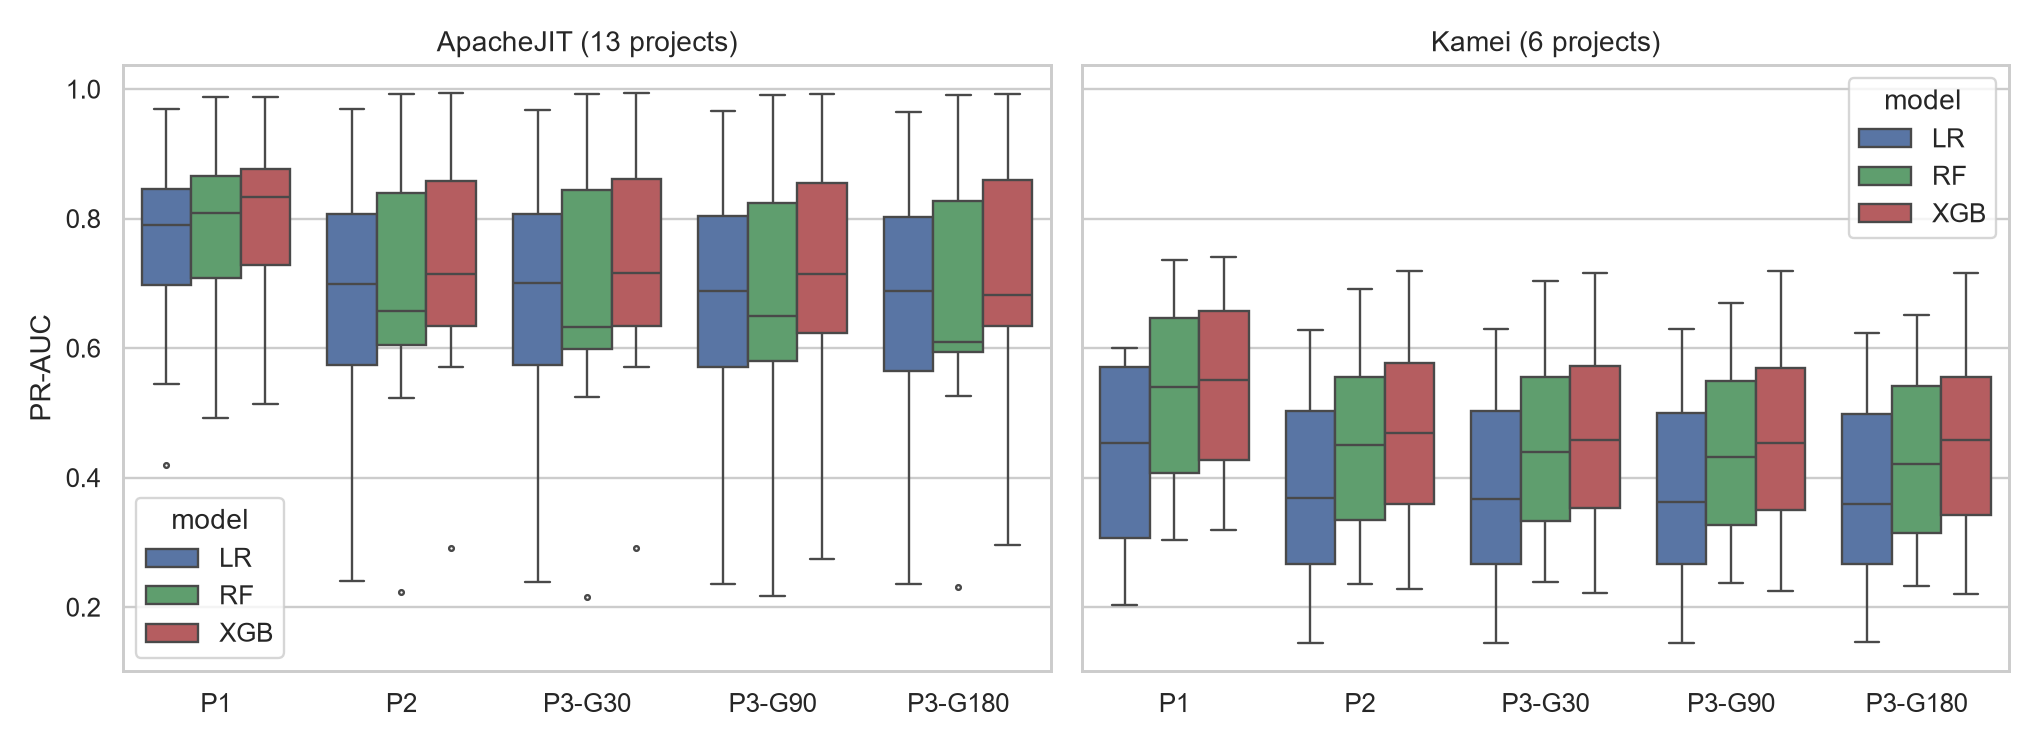
\includegraphics[width=\linewidth]{x_rq1_protocols.png}
\caption{PR-AUC per protocol and model in each dataset (class weighting).}
\label{fig:rq1}
\end{figure}

\paragraph{Hypothesis test.} Table~\ref{tab:rq1tests} reports the paired tests. Over all 57 (project, model) pairs, \pthree{} is significantly lower than P1. The median drop is 0.067 PR-AUC ($\delta=0.22$, small), 0.071 F1 ($\delta=0.24$, small), and 0.088 MCC ($\delta=0.42$, medium), all with $p<0.001$. The result replicates in each dataset. In ApacheJIT the drops are 0.070 PR-AUC, 0.093 F1, and 0.118 MCC (large); in the Kamei data they are 0.063 PR-AUC, 0.044 F1, and 0.025 MCC ($p\le0.009$). It also holds for each model separately over the 19 projects after Holm correction. The PR-AUC drops are 0.059, 0.070, and 0.064 for LR, RF, and XGB (adjusted $p\le0.003$), and the F1 drops are 0.045, 0.077, and 0.087 (adjusted $p\le0.002$). \textbf{H1 is supported in both datasets.}

\begin{table}[t]
\centering
\caption{Paired one-sided Wilcoxon tests ($\Delta$ = median paired difference, first minus second protocol; $n$ = (project, model) pairs).}
\label{tab:rq1tests}
\small
\begin{tabular}{lllrrrl}
\toprule
Scope & Comparison & Metric & $\Delta$ & $p$ & Cliff's $\delta$ & Magnitude \\
\midrule
All ($n=57$) & P1 vs.\ \pthree{} (H1) & PR-AUC & 0.067 & $<$0.001 & 0.215 & small \\
             &                        & F1     & 0.071 & $<$0.001 & 0.237 & small \\
             &                        & MCC    & 0.088 & $<$0.001 & 0.420 & medium \\
             &                        & Lift   & $-$0.110 & 0.993 & $-$0.112 & negligible \\
             & P1 vs.\ P2 (time order) & PR-AUC & 0.064 & $<$0.001 & 0.200 & small \\
             & P2 vs.\ \pthree{} (gap)  & PR-AUC & 0.003 & $<$0.001 & 0.026 & negligible \\
\midrule
ApacheJIT ($n=39$) & P1 vs.\ \pthree{} & PR-AUC & 0.070 & $<$0.001 & 0.256 & small \\
                   &                   & F1     & 0.093 & $<$0.001 & 0.278 & small \\
                   &                   & Lift   & $-$0.132 & 0.983 & $-$0.108 & negligible \\
\midrule
Kamei ($n=18$) & P1 vs.\ \pthree{} & PR-AUC & 0.063 & $<$0.001 & 0.228 & small \\
               &                   & F1     & 0.044 & $<$0.001 & 0.228 & small \\
               &                   & Lift   & $-$0.067 & 0.894 & $-$0.080 & negligible \\
\bottomrule
\end{tabular}
\end{table}

\paragraph{Decomposition and sensitivity.} The P1$\to$P2 step accounts for almost the entire drop (0.064 PR-AUC over all pairs). Adding the latency gap (P2$\to$\pthree) lowers PR-AUC by a statistically significant but negligible 0.003. A 30-day gap is indistinguishable from P2. A 180-day gap gives the largest additional drop (e.g.\ RF 0.657$\to$0.610 in ApacheJIT and 0.451$\to$0.422 in the Kamei data), whereas XGB and LR change by at most 0.03. Withholding more commits removes the most recent, and most relevant, training data, and the cost depends on how fast a project changes.

\paragraph{The role of label maturity.} The drop is uneven across projects (Appendix, Tables~\ref{tab:perproject} and~\ref{tab:perprojectk}). For XGB it ranges from $-0.09$ (\texttt{ignite}, where P3 scores \emph{higher}) to $+0.24$ (\texttt{camel}). Figure~\ref{fig:prev} relates the drop to the ratio between the test prevalence under \pthree{} and under P1. Over the 19 projects the two are strongly correlated for every model (Spearman $\rho=-0.73$, $-0.74$, and $-0.76$ for LR, RF, and XGB; $p\le0.0004$). The correlation is strongest in ApacheJIT ($\rho$ between $-0.84$ and $-0.87$). In the Kamei data, test prevalence also falls in five of the six projects, and the one project whose prevalence does not change (\texttt{platform}) shows no drop. With only six projects, however, the correlation is not significant there ($\rho$ between $-0.09$ and $-0.49$). Consistent with this picture, PR-AUC \emph{lift}, which normalises for prevalence, is not lower under \pthree{} than under P1 in either dataset (Table~\ref{tab:rq1tests}).

\begin{figure}[t]
\centering
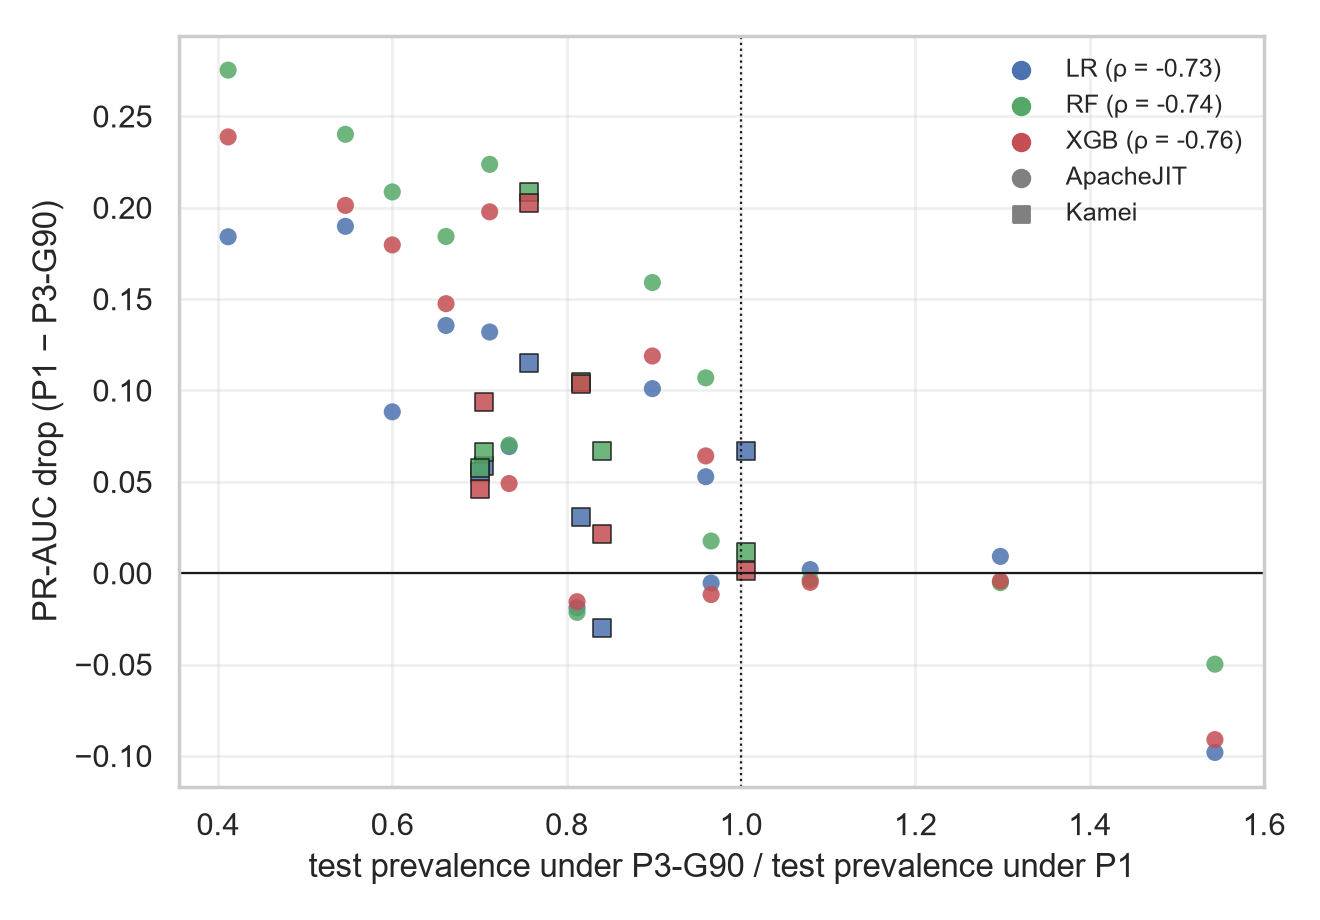
\includegraphics[width=0.66\linewidth]{x_rq1_drop_vs_prevalence.png}
\caption{Per-project PR-AUC drop from P1 to \pthree{} against the change in test prevalence (circles: ApacheJIT; squares: Kamei et al.). Points left of the dotted line are projects whose recent commits carry fewer defect labels.}
\label{fig:prev}
\end{figure}

\paragraph{Same commits, different order.} The paired windows remove differences in test-set composition. Over 1{,}485 pairs (495 windows $\times$ 3 models), the shuffled split still scores significantly higher than the time-ordered one, but by less: the paired difference is 0.024 PR-AUC ($p<0.001$, $\delta=0.07$), 0.025 F1 ($\delta=0.09$), and 0.025 lift ($p<0.001$, $\delta=0.06$), all negligible. The datasets differ here. In ApacheJIT the penalty on identical commits is small (0.019 PR-AUC) and the lift difference is not significant ($p=0.072$). In the Kamei data it is larger (0.037 PR-AUC, $\delta=0.15$; 0.033 F1, $\delta=0.18$, small), and lift also drops (0.109, $p<0.001$). So in the older, multi-language dataset, a genuine time-order penalty remains after prevalence is controlled for.

\finding{1}{Random splitting overstates JIT-SDP performance in both datasets. Over 19 projects, replacing it with \pthree{} lowers median PR-AUC by 0.067, F1 by 0.071, and MCC by 0.088 (H1 supported). The cause is time ordering; the latency gap adds little. The size of the penalty largely follows the lower observed prevalence of recent commits, and prevalence-normalised PR-AUC does not drop. On identical commits a smaller genuine time-order penalty remains, from 0.02 PR-AUC in ApacheJIT to 0.04 in the Kamei data.}

\subsection{RQ2: Imbalance strategies, models, and baselines}\label{sec:rq2}

\paragraph{Imbalance strategies.} Table~\ref{tab:imb} summarises the comparison under \pthree. Over all 57 pairs, class weighting does not increase recall over no treatment (one-sided $p=0.977$). Its effect on F1 is at the edge of significance ($p=0.058$, $\Delta=0.002$), and it does not change PR-AUC ($p=0.080$). Under-sampling does not increase recall or F1 either, and it slightly lowers PR-AUC ($\Delta=-0.004$, $p<0.001$, negligible). The datasets differ in one respect. In the more imbalanced Kamei data (prevalence 3.7--39\%), both treatments slightly improve F1 (weighting $+0.010$, $p=0.024$; under-sampling $+0.012$, $p=0.002$) and MCC ($p\le0.018$), with negligible to small effects, but neither improves recall. \textbf{H2(a) is not supported}, because recall never improves. Each strategy is paired with a threshold chosen on validation data, and that threshold already compensates for most of the class imbalance.

\begin{table}[t]
\centering
\caption{Imbalance strategies under \pthree{}: Wilcoxon tests against no treatment ($\Delta$ = median paired difference).}
\label{tab:imb}
\small
\begin{tabular}{lllrrrl}
\toprule
Scope & Strategy & Metric & $\Delta$ & $p$ & Cliff's $\delta$ & Magnitude \\
\midrule
All ($n=57$) & weight & Recall (one-sided) & $-$0.009 & 0.977 & $-$0.041 & negligible \\
             & weight & F1 (one-sided)     & 0.002 & 0.058 & 0.017 & negligible \\
             & weight & PR-AUC             & 0.000 & 0.080 & $-$0.015 & negligible \\
             & under  & Recall (one-sided) & $-$0.003 & 0.889 & $-$0.053 & negligible \\
             & under  & PR-AUC             & $-$0.004 & $<$0.001 & $-$0.029 & negligible \\
\midrule
Kamei ($n=18$) & weight & F1 (one-sided) & 0.010 & 0.024 & 0.043 & negligible \\
               & weight & MCC            & 0.012 & 0.018 & 0.117 & negligible \\
               & under  & F1 (one-sided) & 0.012 & 0.002 & 0.093 & negligible \\
               & under  & MCC            & 0.014 & 0.007 & 0.198 & small \\
\bottomrule
\end{tabular}
\end{table}

\paragraph{Models.} On PR-AUC over the 19 projects, the Friedman test rejects equal performance of the five rankers ($\chi^2=68.00$, $p<0.001$; Nemenyi CD $=1.40$). The average ranks are XGB 1.21, RF 2.32, LR 2.47, prevalence 4.00, and inverse churn 5.00 (Figure~\ref{fig:ranks}, left). XGB is best in both datasets (average rank 1.23 in ApacheJIT and 1.17 in the Kamei data). It is significantly better than both baselines, but its advantage over RF and LR is smaller than the CD. Table~\ref{tab:pooled} gives the pooled results. In ApacheJIT, XGB reaches PR-AUC 0.771 [95\% CI 0.762--0.779], compared with 0.709 [0.699--0.720] for LR. In the Kamei data, XGB reaches 0.404 [0.393--0.416] and RF 0.391 [0.379--0.403], whereas LR reaches only 0.237 [0.229--0.245], against a chance level of 0.110. The gap between the tree ensembles and LR is therefore much larger in the older, multi-language data.

\begin{figure}[t]
\centering
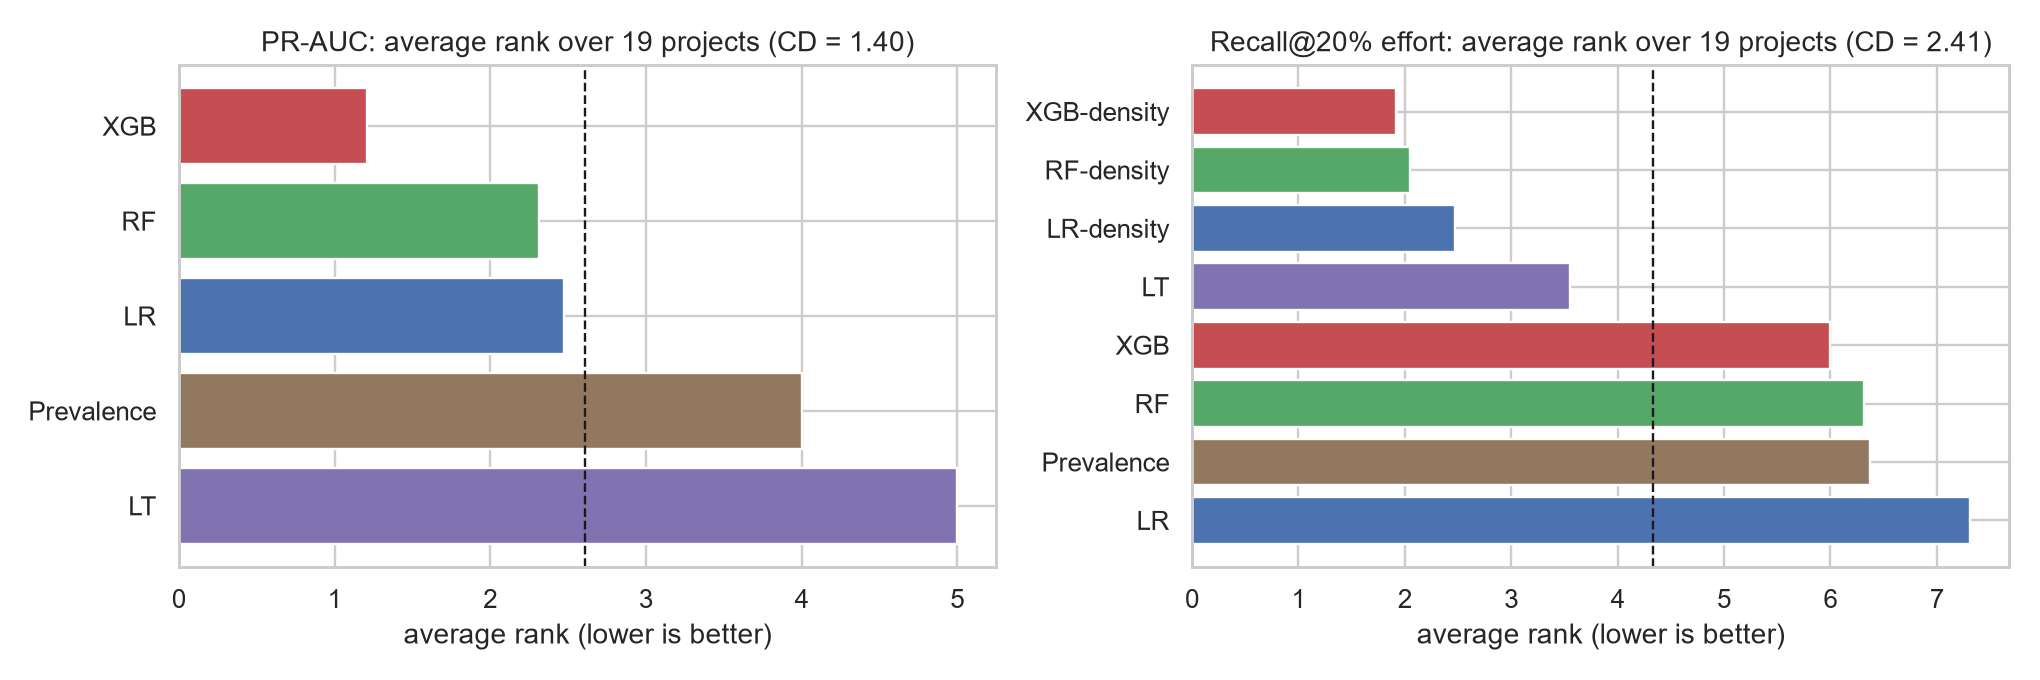
\includegraphics[width=\linewidth]{x_rq2_ranks.png}
\caption{Friedman/Nemenyi average ranks over 19 projects under \pthree{} (lower is better). Left: PR-AUC. Right: Recall@20\% effort, including the density-ranked variants. The dashed line marks the best rank plus the critical difference.}
\label{fig:ranks}
\end{figure}

\begin{table}[t]
\centering
\caption{Pooled \pthree{} results per dataset. PR-AUC with 95\% bootstrap CI; R@20 = Recall@20\% effort (risk ranking / density ranking).}
\label{tab:pooled}
\small
\begin{tabular}{llrrrrr}
\toprule
Dataset & Model & PR-AUC [95\% CI] & F1 & MCC & R@20 risk & R@20 density \\
\midrule
ApacheJIT & LR  & 0.709 [0.699, 0.720] & 0.629 & 0.494 & 0.161 & 0.587 \\
(test prev.\ 0.247) & RF  & 0.760 [0.751, 0.769] & 0.643 & 0.516 & 0.257 & 0.600 \\
          & XGB & 0.771 [0.762, 0.779] & 0.654 & 0.530 & 0.277 & 0.606 \\
          & Prevalence & 0.247 & 0.000 & 0.000 & -- & -- \\
          & Inverse churn & 0.154 & 0.066 & $-$0.287 & 0.561 & 0.561 \\
\midrule
Kamei     & LR  & 0.237 [0.229, 0.245] & 0.331 & 0.236 & 0.340 & 0.648 \\
(test prev.\ 0.110) & RF  & 0.391 [0.379, 0.403] & 0.403 & 0.325 & 0.398 & 0.679 \\
          & XGB & 0.404 [0.393, 0.416] & 0.410 & 0.331 & 0.399 & 0.697 \\
          & Prevalence & 0.110 & 0.000 & 0.000 & -- & -- \\
          & Inverse churn & 0.083 & 0.096 & $-$0.022 & 0.581 & 0.581 \\
\bottomrule
\end{tabular}
\end{table}

\paragraph{Effort-aware ranking.} The picture changes completely when the goal is to find defects with limited review effort. When they rank by raw risk, all three classifiers are far behind the unsupervised inverse-churn baseline on Recall@20\% effort in both datasets: the medians over 19 projects are 0.14--0.25, against 0.59, and the effect is large ($|\delta|\ge0.95$). \textbf{H2(b) is therefore not supported as stated.} Figure~\ref{fig:effort} shows why. High-risk commits are large, and inspecting them first uses up the review budget. When the same models rank commits by risk per changed line, every one of them beats the baseline. Over the 19 projects the medians are 0.621 (LR), 0.630 (RF), and 0.631 (XGB), against 0.588 for the baseline (one-sided $p<0.001$; $\delta=0.31$--$0.34$, small to medium). The advantage is large in the Kamei data (0.656--0.665 vs.\ 0.582; $\delta=0.89$, $p=0.016$, the smallest $p$ attainable with six projects). On the pooled data, density-ranked XGB finds 60.6\% (ApacheJIT) and 69.7\% (Kamei) of defect-inducing commits at 20\% effort, against 56.1\% and 58.1\% for the baseline. The density-ranked variants also take the three best average ranks in the effort Friedman test ($\chi^2=109.81$, $p<0.001$; Figure~\ref{fig:ranks}, right). Their advantage over the baseline is smaller than the conservative Nemenyi CD (2.41), although the paired Wilcoxon tests are significant.

\begin{figure}[t]
\centering
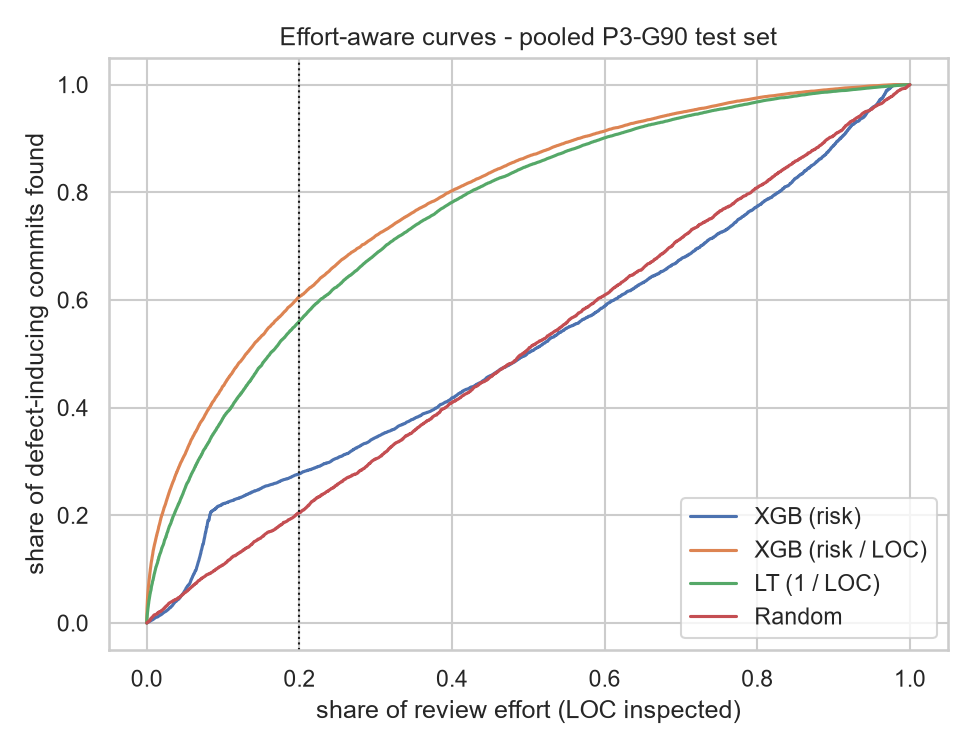
\includegraphics[width=0.58\linewidth]{rq2_effort_curves.png}
\caption{Cumulative share of defect-inducing commits found against the share of churn inspected (pooled ApacheJIT \pthree{} test set). The dotted line marks the 20\% effort budget.}
\label{fig:effort}
\end{figure}

\paragraph{Selection rule.} Following the pre-registered rule, XGB has the best PR-AUC in both datasets. It also has the best density-ranked Recall@20\% effort over the 19 projects and on both pooled test sets, so we select it for the prototype.

\finding{2}{With validation-tuned thresholds, class weighting and under-sampling never improve recall, and they give at most negligible F1 and MCC gains on the more imbalanced data (H2a not supported). XGBoost is the best risk ranker in both datasets. For review prioritisation, supervised models that rank by raw risk lose badly to an inverse-churn baseline (H2b not supported as stated). Ranking by risk per changed line reverses this in every model and in both datasets.}

\subsection{RQ3: Influential features and their stability}\label{sec:rq3}

\paragraph{Global importance.} Change size dominates in both datasets, but the secondary signals differ (Figure~\ref{fig:shap}). For the pooled ApacheJIT XGB model, the most influential features by mean $|\text{SHAP}|$ are lines added (\texttt{la}, 1.03), the \texttt{fix} indicator (0.57), lines deleted (0.25), unique changes (\texttt{nuc}, 0.24), and recent developer experience (\texttt{arexp}, 0.22). For the pooled Kamei model they are the number of files (\texttt{nf}, 0.57), file age (\texttt{age}, 0.50), relative lines added (\texttt{la}, 0.48), \texttt{fix} (0.27), and \texttt{ndev} (0.25). In ApacheJIT the standardised LR model agrees with XGB: its strongest coefficients are \texttt{la} (odds ratio 2.82 per standard deviation), \texttt{fix} (2.11), \texttt{nuc} (1.57), and \texttt{ld} (1.26). Larger changes and bug-fixing changes are riskier in both datasets.

\begin{figure}[t]
\centering
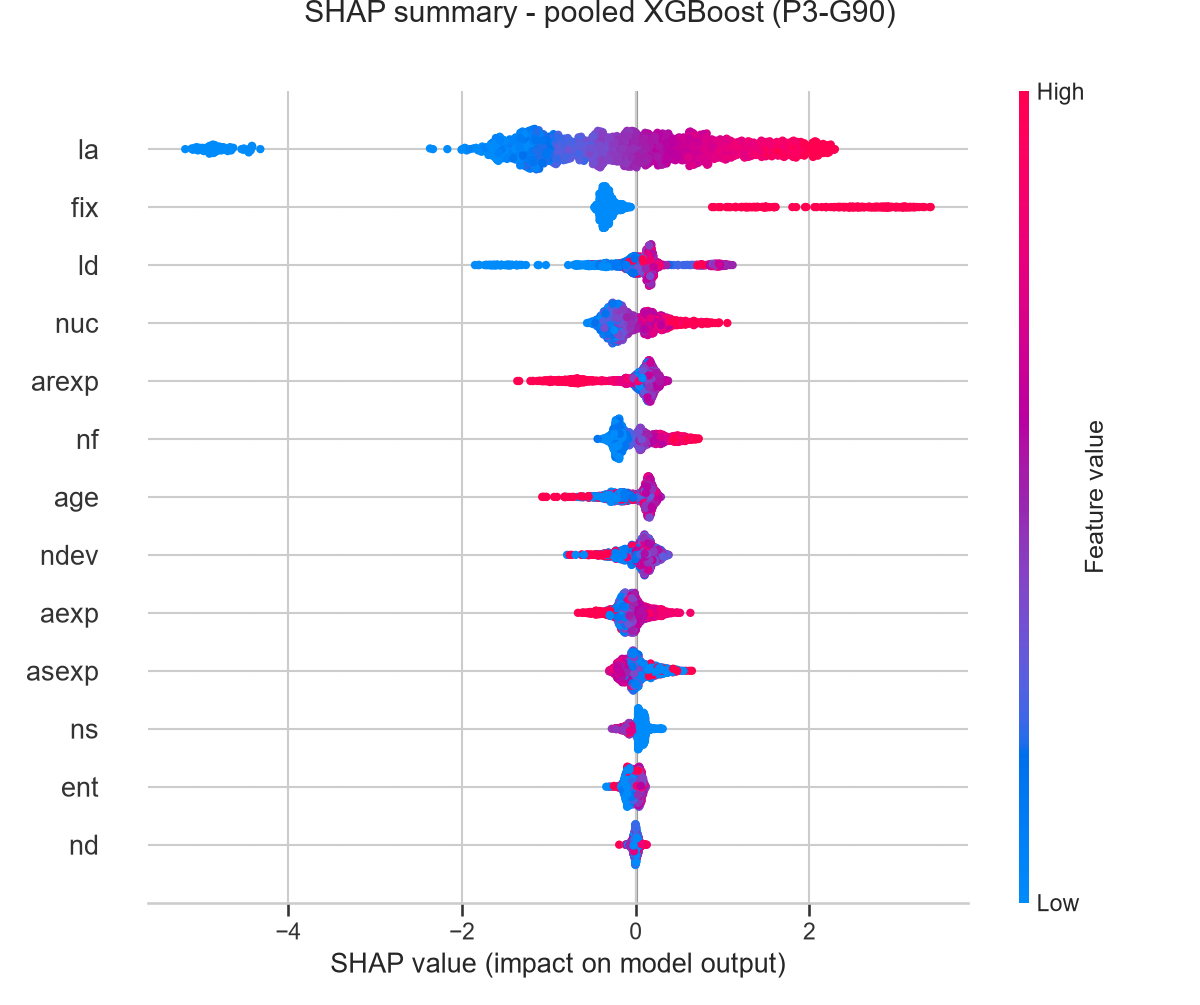
\includegraphics[width=0.49\linewidth]{rq3_shap_beeswarm.png}\hfill
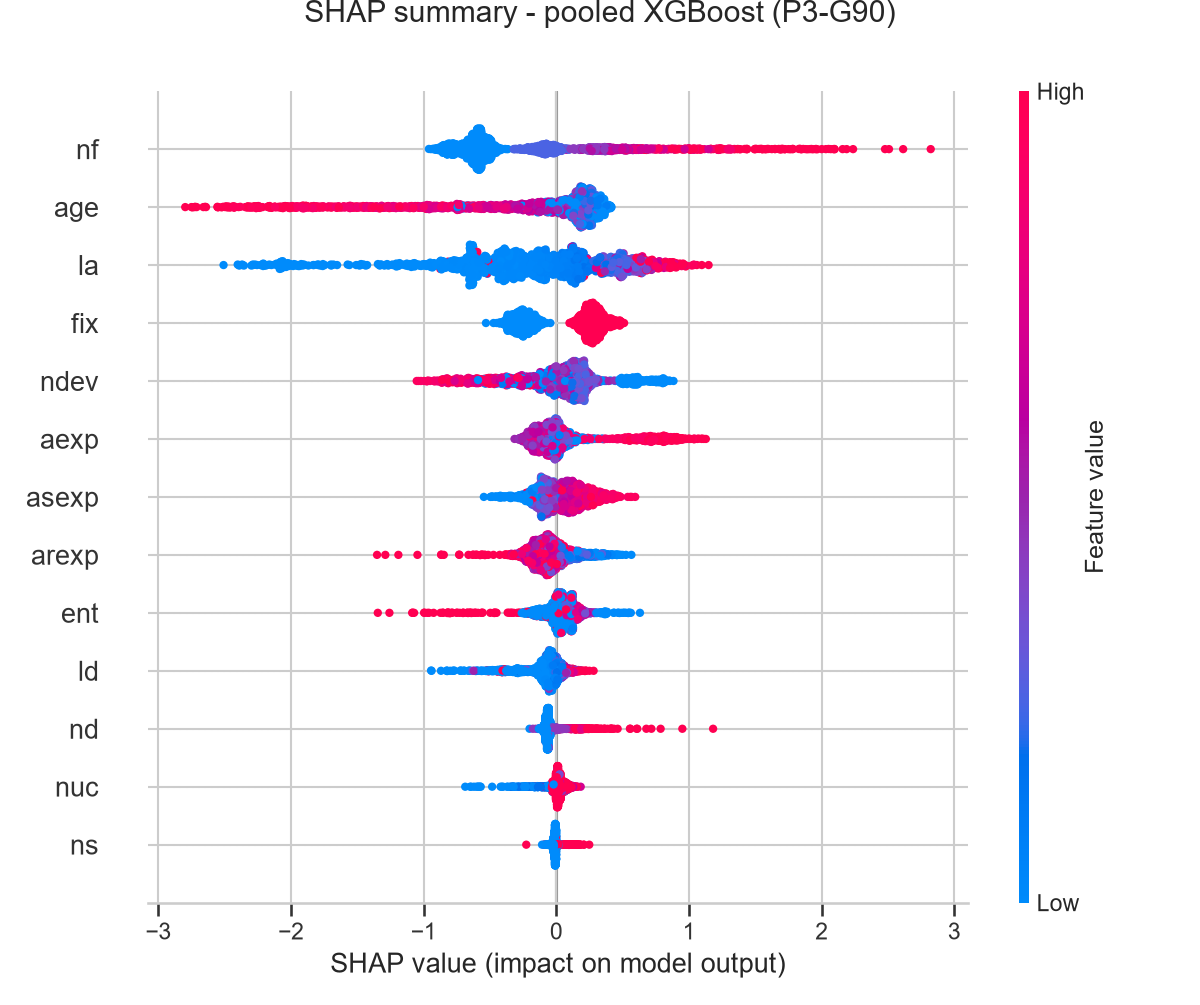
\includegraphics[width=0.49\linewidth]{k_rq3_shap_beeswarm.png}
\caption{SHAP summaries of the pooled \pthree{} XGBoost models (2{,}000 test commits). Left: ApacheJIT; right: Kamei et al.}
\label{fig:shap}
\end{figure}

\paragraph{Temporal stability.} Table~\ref{tab:stab} summarises stability over 476 pairs of consecutive windows. Over both datasets, the median Spearman correlation over the union of the two top-five sets is 0.64, and 43\% of pairs reach 0.7. \textbf{H3 is therefore not supported overall, but the result depends on the dataset.} The Kamei projects meet the threshold (median $\rho=0.71$; 0.91 over all 13 features), whereas ApacheJIT does not (0.60; 0.84 over all features). In both datasets the instability lies below the top. Lines added is in the top five in 100\% (ApacheJIT) and 99\% (Kamei) of windows. The next features are \texttt{ld}, \texttt{fix}, and \texttt{nuc} in ApacheJIT, and \texttt{nf} (93\%) and \texttt{age} (78\%) in the Kamei data. The median top-five Jaccard overlap is 0.67 in both datasets, so typically four of the five features are shared between consecutive windows (Figure~\ref{fig:stab}).

\begin{table}[t]
\centering
\caption{Stability of XGBoost SHAP rankings between consecutive windows (medians).}
\label{tab:stab}
\small
\begin{tabular}{lrrrrr}
\toprule
Dataset & Pairs & $\rho$ (top-5 union) & Share $\ge0.7$ & $\rho$ (all 13) & Jaccard (top-5) \\
\midrule
ApacheJIT & 331 & 0.600 & 38\% & 0.835 & 0.667 \\
Kamei et al. & 145 & 0.714 & 54\% & 0.912 & 0.667 \\
All & 476 & 0.643 & 43\% & 0.854 & 0.667 \\
\bottomrule
\end{tabular}
\end{table}

\begin{figure}[t]
\centering
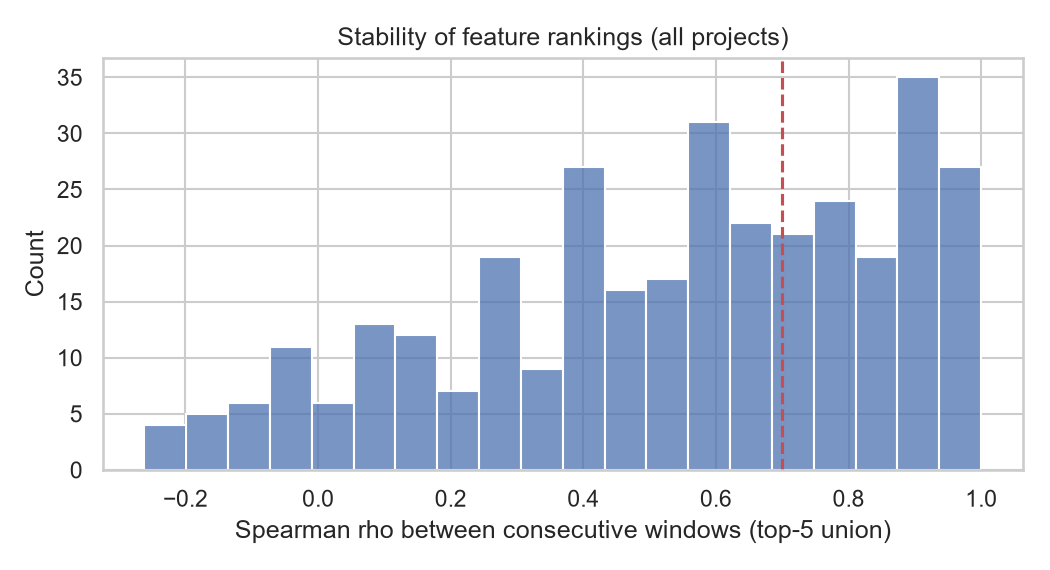
\includegraphics[width=0.49\linewidth]{rq3_stability_hist.png}\hfill
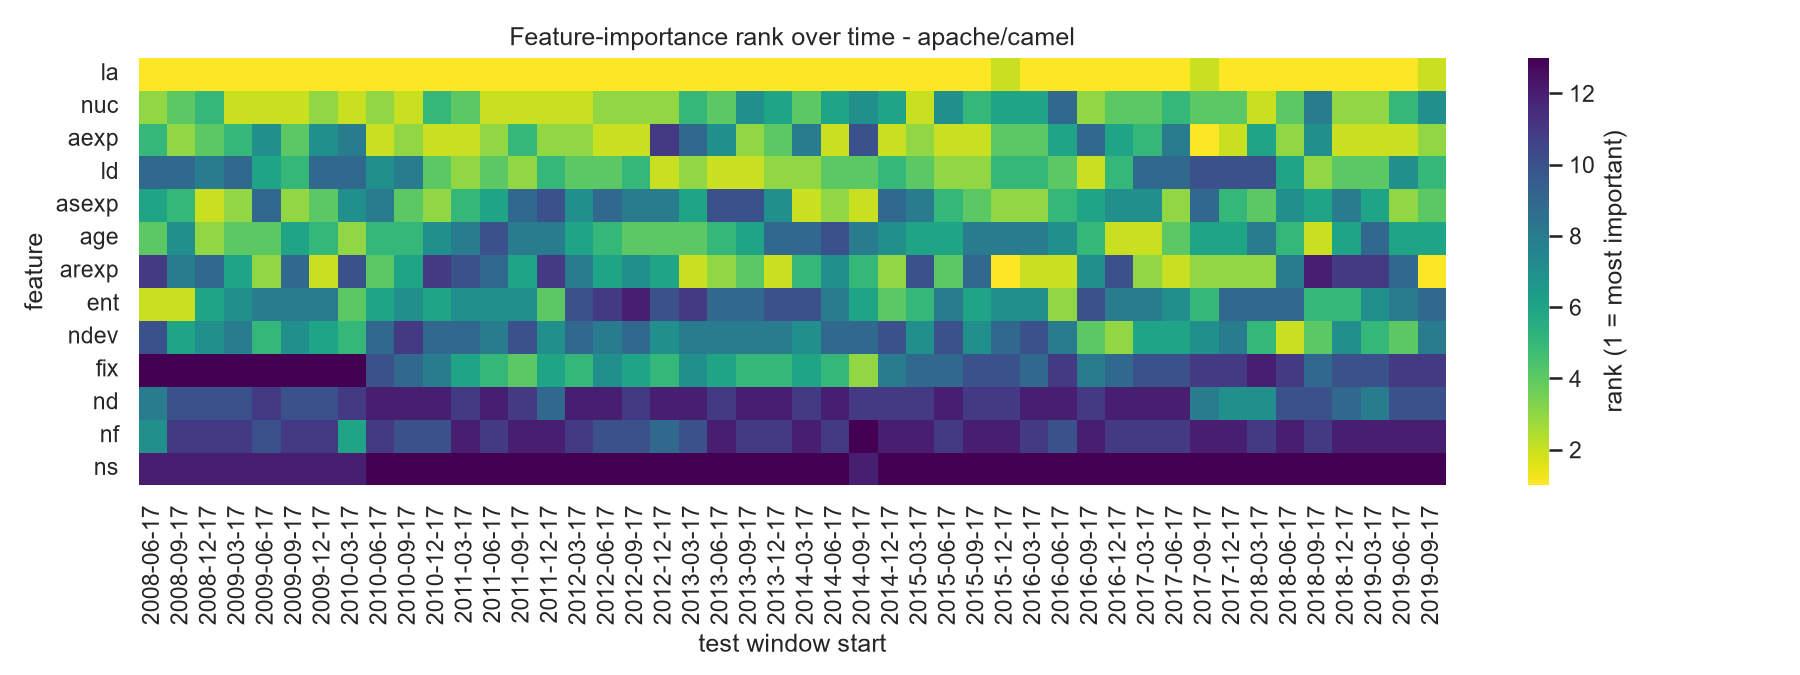
\includegraphics[width=0.49\linewidth]{rq3_rank_heatmap.png}
\caption{ApacheJIT. Left: Spearman $\rho$ of top-five SHAP rankings between consecutive windows (red line: 0.7 threshold). Right: feature rank over time for the project with the most windows (\texttt{camel}).}
\label{fig:stab}
\end{figure}

\finding{3}{Change size is the dominant and stable predictor in both datasets. The ordering of the remaining top features is stable in the older Kamei projects (median $\rho=0.71$) but drifts between three-month windows in ApacheJIT ($\rho=0.60$). H3 is not supported overall and is dataset-dependent, which is in line with the moving-target nature of fix-inducing changes \citep{mcintosh2018}.}

% ===========================================================================
\section{Discussion}\label{sec:discussion}

\paragraph{How much of the realism penalty is real?} The second dataset sharpens the interpretation of RQ1. Like \citet{falessi2020} and \citet{song2023a}, we find that shuffled evaluation produces systematically higher numbers. The penalty would change conclusions in practice. In ApacheJIT, for instance, RF falls from second to third place and loses 0.16 PR-AUC. Three observations show that a large part of the penalty reflects \emph{what is being measured} rather than \emph{how well the model predicts}: the drop correlates with the prevalence shift, PR-AUC lift does not drop in either dataset, and the effect on identical commits is small. Recent commits have fewer observed defects because their defects have not yet been found, so a time-ordered test set is labelled with fewer positives than a shuffled one. The Kamei data adds an important caveat. On identical commits, a genuine penalty of about 0.04 PR-AUC remains there, and lift also drops. Time ordering therefore does make prediction harder, through concept drift, but by less than absolute metrics suggest. Researchers who report absolute PR-AUC under time-ordered evaluation should also report test prevalence and a normalised measure. Otherwise, label immaturity will be read as model weakness.

\paragraph{Is the latency gap worth it?} Removing the last 30--90 days before the cut-off cost almost nothing in either dataset, whereas a 180-day gap cost up to 0.05 PR-AUC. When fix dates are missing, a gap is the correct way to avoid training on immature negatives \citep{cabral2019}. It should be calibrated to the typical time-to-fix of each project rather than set as large as possible, because it trades label correctness for recency.

\paragraph{Imbalance treatment.} With a validation-tuned threshold, neither class weighting nor under-sampling improved recall. Their only benefit was a negligible F1 and MCC gain on the more imbalanced Kamei projects, and under-sampling slightly lowered PR-AUC. Practitioners can safely prioritise threshold selection over resampling. This also avoids the probability shift reported by \citet{tantithamthavorn2020}.

\paragraph{Supervised vs.\ unsupervised effort-aware prediction.} Our results support both sides of the debate started by \citet{yang2016} and continued by \citet{fu2017} and \citet{huang2019}. The inverse-churn baseline is very strong, and it beats every supervised model that ranks by raw risk, in both datasets. This comparison is unfair to supervised models, because raw risk correlates with size. Dividing risk by effort requires no retraining, yet it lets all three supervised models beat the baseline in both datasets, with a large effect on the Kamei data. Effort-aware JIT-SDP studies should therefore always report the density ranking of supervised models next to the unsupervised baseline.

\paragraph{Generalisation across datasets.} The two datasets differ in age, ecosystem, language, labelling pipeline, metric normalisation, and prevalence. The qualitative conclusions are nevertheless the same in both. Random splits overstate performance, the latency gap matters little, rebalancing does not help recall, XGBoost is the best risk ranker, density ranking beats the size baseline, and change size dominates. Two findings are dataset-dependent: how stable the secondary features are, and how large the genuine time-order penalty is. Both are plausibly related to how fast each project evolved.

\paragraph{Implications for practitioners.} (1) Expect lower numbers than published random-split results, estimate performance with time-ordered splits, and monitor test prevalence. (2) Use XGBoost with a validation-tuned threshold; LR is easier to explain but loses much ranking quality on some projects. (3) For review queues, sort commits by risk per changed line. (4) Retrain periodically and monitor SHAP rankings, because secondary signals can drift within months.

\paragraph{Implications for researchers.} (1) Use time-ordered protocols and report the prevalence of each test set. (2) Use paired designs on identical commits to isolate the effect of time order. (3) Report prevalence-normalised metrics alongside PR-AUC. (4) Treat the latency gap as a sensitivity parameter. (5) Replicate on datasets with different labelling pipelines before generalising.

% ===========================================================================
\section{Threats to Validity}\label{sec:threats}

\paragraph{Construct validity.} Labels in both datasets come from SZZ variants and are noisy \citep{herbold2022}; we reuse public datasets and do not claim ground truth. Effort is approximated by churn, which simplifies real review effort. In the Kamei data, churn is reconstructed from normalised values, and commits that create new files have zero LT and therefore minimal effort. Without fix timestamps, label latency is approximated by a gap. We mitigate this with three gap sizes, but per-commit label masking would be more precise. Feature definitions differ slightly between the datasets (e.g.\ normalised churn and \texttt{nuc} in the Kamei data), so we never mix the datasets in a model and compare them only at the level of conclusions.

\paragraph{Internal validity.} Leakage is controlled by automated checks and unit tests. Preprocessing is fitted on training data only, and thresholds are chosen on validation data. Rolling windows use fixed hyper-parameters, which may slightly underestimate tuned performance in both members of each pair; because the comparison is paired, the effect on the contrast should be limited. The \texttt{fix} indicator is assumed to be known at commit time. If a project assigns issue links after the commit, the indicator could carry mild leakage.

\paragraph{Conclusion validity.} We use non-parametric paired tests, Holm correction for per-model families, effect sizes, three random seeds for P1, 495 windows, and bootstrap confidence intervals, and we report every test over all projects and per dataset. With six projects, per-dataset tests on the Kamei data have limited power: the smallest attainable one-sided $p$ is 0.016, and correlations over six points are unstable. The Nemenyi test is conservative and cannot separate close models.

\paragraph{External validity.} The two datasets cover 19 open-source projects in four languages and two decades. Results may still differ in industrial settings or in ecosystems such as Python or JavaScript. Two ApacheJIT projects were excluded by a pre-registered rule.

% ===========================================================================
\section{Conclusion}\label{sec:conclusion}

We measured how realistic evaluation changes the conclusions drawn about standard JIT-SDP classifiers on 321{,}288 commits from 19 projects in two independent datasets. Random splitting overstates PR-AUC, F1, and MCC in both datasets, and the overstatement comes from ignoring time order rather than from the label-latency gap. A large part of the measured gap is explained by the lower observed defect prevalence of recent commits, and prevalence-normalised PR-AUC does not drop. On identical commits, however, a smaller genuine penalty remains, and it is larger in the older multi-language dataset. With validation-tuned thresholds, imbalance treatments do not improve recall. XGBoost is the best risk ranker, but supervised models beat a simple size baseline for review prioritisation only when they rank by risk per changed line, which they then do consistently. Change size is the dominant predictor everywhere, while the stability of the other top features depends on the dataset.

Future work will use repositories with fix timestamps to replace the gap with per-commit label masking, extend the study to further ecosystems and industrial data, and evaluate online learners that adapt to the observed drift.

% ===========================================================================
\section*{Declarations}

\paragraph{Data availability.} ApacheJIT is publicly available at \url{https://github.com/hosseinkshvrz/apachejit}. The dataset of \citet{kamei2013} is available in the replication package of \citet{fu2017} at \url{https://github.com/WeiFoo/RevisitUnsupervised}. The complete replication package (code, configuration, raw results, figures, unit tests, and the prototype) will be made available in a public repository upon acceptance \texttt{[repository URL]}.

\paragraph{Funding.} The authors did not receive funding for this work.

\paragraph{Competing interests.} The authors declare no competing interests.

\paragraph{Use of AI tools.} AI-based assistants were used to help implement the experiment code, generate figures, and edit the language of this manuscript. The authors designed the study, reviewed all code and results, verified every reported number against the generated outputs, and take full responsibility for the content.

\paragraph{Author contributions (CRediT).} F.\ H.\ Ghariani and A.\ K.\ Almuqadimi: Conceptualization, Methodology, Software, Formal analysis, Writing -- original draft, Writing -- review \& editing. \texttt{[Adjust as appropriate.]}

\paragraph{Acknowledgements.} We thank Dr.\ Mohamed Alardawi (College of Computer Technology, Tripoli) for supervising this work. We also thank the authors of ApacheJIT and of the Kamei et al.\ dataset, and Yang et al.\ and Fu and Menzies, for making their data public.

% ===========================================================================
\bibliographystyle{plainnat}
\bibliography{references}

% ===========================================================================
\appendix
\section{Per-project results}\label{app:perproject}

\begin{table}[h]
\centering
\caption{ApacheJIT: XGBoost PR-AUC per project and protocol, with training and test prevalence of the chronological split.}
\label{tab:perproject}
\small
\begin{tabular}{lrrrrrrr}
\toprule
Project & P1 & P2 & P3\textsubscript{G30} & P3\textsubscript{G90} & P3\textsubscript{G180} & Prev.\ train & Prev.\ test \\
\midrule
activemq          & 0.668 & 0.616 & 0.617 & 0.604 & 0.595 & 0.233 & 0.220 \\
camel             & 0.513 & 0.291 & 0.292 & 0.274 & 0.297 & 0.170 & 0.056 \\
cassandra         & 0.844 & 0.858 & 0.861 & 0.856 & 0.859 & 0.388 & 0.369 \\
flink             & 0.764 & 0.570 & 0.571 & 0.567 & 0.565 & 0.270 & 0.171 \\
groovy            & 0.607 & 0.634 & 0.635 & 0.623 & 0.633 & 0.216 & 0.163 \\
hadoop-hdfs       & 0.987 & 0.994 & 0.994 & 0.992 & 0.992 & 0.738 & 0.825 \\
hadoop-mapreduce  & 0.965 & 0.970 & 0.973 & 0.970 & 0.975 & 0.553 & 0.824 \\
hbase             & 0.867 & 0.724 & 0.720 & 0.720 & 0.710 & 0.496 & 0.287 \\
hive              & 0.944 & 0.893 & 0.893 & 0.894 & 0.886 & 0.688 & 0.453 \\
ignite            & 0.729 & 0.818 & 0.812 & 0.820 & 0.815 & 0.155 & 0.313 \\
kafka             & 0.877 & 0.689 & 0.690 & 0.675 & 0.662 & 0.559 & 0.256 \\
spark             & 0.820 & 0.641 & 0.640 & 0.640 & 0.641 & 0.505 & 0.259 \\
zeppelin          & 0.834 & 0.715 & 0.716 & 0.715 & 0.682 & 0.447 & 0.385 \\
\bottomrule
\end{tabular}
\end{table}

\begin{table}[h]
\centering
\caption{Kamei et al.: XGBoost PR-AUC per project and protocol, with training and test prevalence of the chronological split.}
\label{tab:perprojectk}
\small
\begin{tabular}{lrrrrrrr}
\toprule
Project & P1 & P2 & P3\textsubscript{G30} & P3\textsubscript{G90} & P3\textsubscript{G180} & Prev.\ train & Prev.\ test \\
\midrule
bugzilla (Perl)   & 0.740 & 0.720 & 0.717 & 0.719 & 0.715 & 0.392 & 0.309 \\
columba (Java)    & 0.659 & 0.483 & 0.462 & 0.457 & 0.467 & 0.337 & 0.231 \\
jdt (Java)        & 0.420 & 0.328 & 0.321 & 0.316 & 0.307 & 0.155 & 0.117 \\
mozilla (C++)     & 0.319 & 0.227 & 0.223 & 0.225 & 0.220 & 0.059 & 0.037 \\
platform (Java)   & 0.451 & 0.455 & 0.453 & 0.449 & 0.448 & 0.147 & 0.148 \\
postgres (C)      & 0.653 & 0.608 & 0.609 & 0.607 & 0.584 & 0.283 & 0.176 \\
\bottomrule
\end{tabular}
\end{table}

\end{document}
